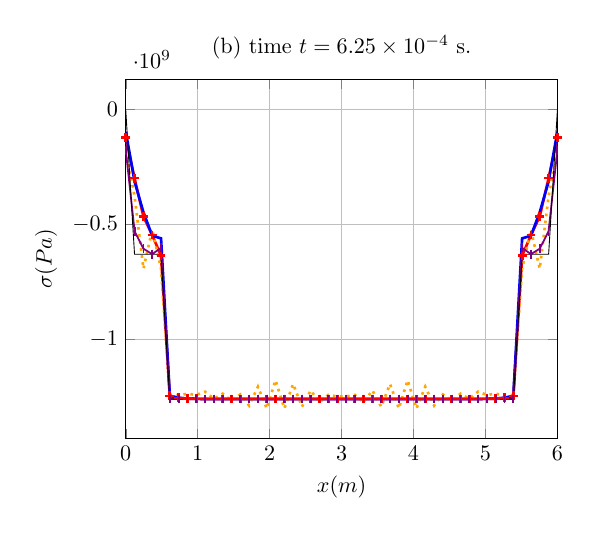
\begin{tikzpicture}[scale=0.8]
\begin{axis}[xlabel=$x (m)$,ylabel=$\sigma (Pa)$,ymajorgrids=true,xmajorgrids=true,legend pos=outer north east,title={(b) time $t = 6.25\times 10^{-4} $ s.},xmin=0.,xmax=6.]
\addplot[Red,very thick,mark=+,solid] coordinates {(0.0,-120597397.19248778) (0.12244897959183673,-298539345.15508544) (0.24489795918367346,-464504460.170754) (0.36734693877551017,-546627376.3559334) (0.4897959183673469,-635546108.2543886) (0.6122448979591837,-1247334335.3333962) (0.7346938775510203,-1255980074.5990539) (0.8571428571428571,-1259371705.5275755) (0.9795918367346939,-1260535220.1287405) (1.1020408163265305,-1260885267.5005968) (1.2244897959183674,-1260977777.705495) (1.346938775510204,-1260999265.6570995) (1.4693877551020407,-1261003650.0375175) (1.5918367346938775,-1261004434.5740557) (1.7142857142857142,-1261004557.3391547) (1.836734693877551,-1261004574.0682204) (1.9591836734693877,-1261004576.0419452) (2.0816326530612246,-1261004576.241996) (2.204081632653061,-1261004576.2592359) (2.326530612244898,-1261004576.260481) (2.4489795918367347,-1261004576.260556) (2.571428571428571,-1261004576.2605588) (2.693877551020408,-1261004576.260559) (2.816326530612245,-1261004576.2605588) (2.9387755102040813,-1261004576.260559) (3.061224489795918,-1261004576.2605584) (3.183673469387755,-1261004576.2605586) (3.306122448979592,-1261004576.2605588) (3.4285714285714284,-1261004576.2605581) (3.5510204081632653,-1261004576.2605555) (3.673469387755102,-1261004576.260481) (3.7959183673469385,-1261004576.2592354) (3.9183673469387754,-1261004576.2419953) (4.040816326530612,-1261004576.0419443) (4.163265306122449,-1261004574.06822) (4.285714285714286,-1261004557.3391542) (4.408163265306122,-1261004434.5740552) (4.530612244897959,-1261003650.037517) (4.653061224489796,-1260999265.6570988) (4.775510204081632,-1260977777.7054946) (4.8979591836734695,-1260885267.500596) (5.020408163265306,-1260535220.1287398) (5.142857142857142,-1259371705.5275738) (5.26530612244898,-1255980074.5990536) (5.387755102040816,-1247334335.3333952) (5.5102040816326525,-635546108.2543867) (5.63265306122449,-546627376.3559326) (5.755102040816326,-464504460.1707534) (5.877551020408163,-298539345.15508515) (6.0,-120597397.19248791) };
\addplot[Orange,very thick,mark=none,dotted] coordinates {(0.0011999999999999927,-176853791.94554004) (0.12359999999999997,-378394340.717152) (0.24599999999999994,-693239198.8311979) (0.36839999999999995,-523439989.89111507) (0.4907999999999999,-693552985.1722431) (0.6131999999999999,-1243921088.325841) (0.7355999999999999,-1243896835.4237814) (0.858,-1238512519.7129703) (0.9803999999999998,-1242876003.1599257) (1.1027999999999998,-1229134621.6433644) (1.2251999999999996,-1260098267.149167) (1.3475999999999997,-1238022210.520185) (1.4699999999999998,-1269111852.1192086) (1.5923999999999996,-1241379610.2251832) (1.7147999999999997,-1289870286.8459477) (1.8371999999999995,-1207539167.6018116) (1.9595999999999996,-1302352875.6492124) (2.0819999999999994,-1179646467.1836338) (2.2043999999999997,-1302099080.7920847) (2.3267999999999995,-1195754724.162506) (2.4491999999999994,-1294783662.9363751) (2.5715999999999997,-1223699568.3092146) (2.6939999999999995,-1275816869.6395779) (2.8163999999999993,-1243094391.3994842) (2.9387999999999996,-1250401942.2614183) (3.0611999999999995,-1250401942.2613835) (3.1835999999999993,-1243094391.3995185) (3.305999999999999,-1275816869.6395504) (3.4283999999999994,-1223699568.3092418) (3.5507999999999993,-1294783662.9363482) (3.673199999999999,-1195754724.16253) (3.7955999999999994,-1302099080.7920847) (3.9179999999999993,-1179646467.1836205) (4.040399999999999,-1302352875.6492195) (4.1628,-1207539167.601786) (4.2852,-1289870286.8459682) (4.4076,-1241379610.2251687) (4.53,-1269111852.1192243) (4.6524,-1238022210.5201812) (4.7748,-1260098267.1491652) (4.8972,-1229134621.643366) (5.0196,-1242876003.159929) (5.142,-1238512519.712955) (5.2644,-1243896835.4238017) (5.3868,-1243921088.3258262) (5.5092,-693552985.1722746) (5.6316,-523439989.8910899) (5.754,-693239198.8312114) (5.8764,-378394340.71715474) (5.9988,-176853791.9455247) };
\addplot[Blue,very thick,mark=none,solid] coordinates {(0.0011999999999999927,-96650988.15728289) (0.12359999999999997,-314215597.0101885) (0.24599999999999994,-447225867.04361707) (0.36839999999999995,-549691260.4581364) (0.4907999999999999,-561200942.1999743) (0.6131999999999999,-1247334335.3333952) (0.7355999999999999,-1255980074.5990531) (0.858,-1259371705.5275743) (0.9803999999999998,-1260535220.1287396) (1.1027999999999998,-1260885267.5005958) (1.2251999999999996,-1260977777.7054944) (1.3475999999999997,-1260999265.6570985) (1.4699999999999998,-1261003650.037517) (1.5923999999999996,-1261004434.5740547) (1.7147999999999997,-1261004557.3391533) (1.8371999999999995,-1261004574.0682194) (1.9595999999999996,-1261004576.041944) (2.0819999999999994,-1261004576.2419949) (2.2043999999999997,-1261004576.259235) (2.3267999999999995,-1261004576.260481) (2.4491999999999994,-1261004576.2605555) (2.5715999999999997,-1261004576.2605588) (2.6939999999999995,-1261004576.2605588) (2.8163999999999993,-1261004576.2605588) (2.9387999999999996,-1261004576.260559) (3.0611999999999995,-1261004576.2605588) (3.1835999999999993,-1261004576.260559) (3.305999999999999,-1261004576.260559) (3.4283999999999994,-1261004576.260559) (3.5507999999999993,-1261004576.2605555) (3.673199999999999,-1261004576.2604809) (3.7955999999999994,-1261004576.2592351) (3.9179999999999993,-1261004576.241995) (4.040399999999999,-1261004576.041944) (4.1628,-1261004574.0682197) (4.2852,-1261004557.3391535) (4.4076,-1261004434.5740547) (4.53,-1261003650.0375168) (4.6524,-1260999265.6570985) (4.7748,-1260977777.7054942) (4.8972,-1260885267.5005958) (5.0196,-1260535220.1287396) (5.142,-1259371705.5275743) (5.2644,-1255980074.5990531) (5.3868,-1247334335.333395) (5.5092,-561200942.1999743) (5.6316,-549691260.4581364) (5.754,-447225867.0436171) (5.8764,-314215597.0101884) (5.9988,-96650988.15728283) };
\addplot[Purple,thick,mark=|,solid] coordinates {(0.0011999999999999927,-178085389.46677893) (0.12359999999999997,-530375739.95348394) (0.24599999999999994,-606212710.479109) (0.36839999999999995,-629775762.9786947) (0.4907999999999999,-602317892.3964041) (0.6131999999999999,-1261002720.0436904) (0.7355999999999999,-1261004493.0577958) (0.858,-1261004572.8496082) (0.9803999999999998,-1261004576.1336117) (1.1027999999999998,-1261004576.256299) (1.2251999999999996,-1261004576.2604308) (1.3475999999999997,-1261004576.2605557) (1.4699999999999998,-1261004576.260559) (1.5923999999999996,-1261004576.2605586) (1.7147999999999997,-1261004576.2605586) (1.8371999999999995,-1261004576.260559) (1.9595999999999996,-1261004576.260559) (2.0819999999999994,-1261004576.2605586) (2.2043999999999997,-1261004576.2605588) (2.3267999999999995,-1261004576.2605588) (2.4491999999999994,-1261004576.2605588) (2.5715999999999997,-1261004576.2605586) (2.6939999999999995,-1261004576.2605588) (2.8163999999999993,-1261004576.2605586) (2.9387999999999996,-1261004576.2605588) (3.0611999999999995,-1261004576.2605588) (3.1835999999999993,-1261004576.260559) (3.305999999999999,-1261004576.2605584) (3.4283999999999994,-1261004576.2605584) (3.5507999999999993,-1261004576.2605586) (3.673199999999999,-1261004576.2605588) (3.7955999999999994,-1261004576.2605588) (3.9179999999999993,-1261004576.260559) (4.040399999999999,-1261004576.2605586) (4.1628,-1261004576.2605588) (4.2852,-1261004576.2605586) (4.4076,-1261004576.2605586) (4.53,-1261004576.2605586) (4.6524,-1261004576.2605553) (4.7748,-1261004576.2604303) (4.8972,-1261004576.2562997) (5.0196,-1261004576.133612) (5.142,-1261004572.8496091) (5.2644,-1261004493.0577967) (5.3868,-1261002720.0436902) (5.5092,-602317892.3964037) (5.6316,-629775762.9786928) (5.754,-606212710.4791106) (5.8764,-530375739.9534838) (5.9988,-178085389.4667765) };
\addplot[black,thin,mark=none,solid] coordinates {(0.0,-0.0) (0.12244897959183673,-630502288.1302795) (0.24489795918367346,-630502288.1302795) (0.36734693877551017,-630502288.1302795) (0.4897959183673469,-630502288.1302795) (0.6122448979591837,-1261004576.260559) (0.7346938775510203,-1261004576.260559) (0.8571428571428571,-1261004576.260559) (0.9795918367346939,-1261004576.260559) (1.1020408163265305,-1261004576.260559) (1.2244897959183674,-1261004576.260559) (1.346938775510204,-1261004576.260559) (1.4693877551020407,-1261004576.260559) (1.5918367346938775,-1261004576.260559) (1.7142857142857142,-1261004576.260559) (1.836734693877551,-1261004576.260559) (1.9591836734693877,-1261004576.260559) (2.0816326530612246,-1261004576.260559) (2.204081632653061,-1261004576.260559) (2.326530612244898,-1261004576.260559) (2.4489795918367347,-1261004576.260559) (2.571428571428571,-1261004576.260559) (2.693877551020408,-1261004576.260559) (2.816326530612245,-1261004576.260559) (2.9387755102040813,-1261004576.260559) (3.061224489795918,-1261004576.260559) (3.183673469387755,-1261004576.260559) (3.306122448979592,-1261004576.260559) (3.4285714285714284,-1261004576.260559) (3.5510204081632653,-1261004576.260559) (3.673469387755102,-1261004576.260559) (3.7959183673469385,-1261004576.260559) (3.9183673469387754,-1261004576.260559) (4.040816326530612,-1261004576.260559) (4.163265306122449,-1261004576.260559) (4.285714285714286,-1261004576.260559) (4.408163265306122,-1261004576.260559) (4.530612244897959,-1261004576.260559) (4.653061224489796,-1261004576.260559) (4.775510204081632,-1261004576.260559) (4.8979591836734695,-1261004576.260559) (5.020408163265306,-1261004576.260559) (5.142857142857142,-1261004576.260559) (5.26530612244898,-1261004576.260559) (5.387755102040816,-1261004576.260559) (5.5102040816326525,-630502288.1302795) (5.63265306122449,-630502288.1302795) (5.755102040816326,-630502288.1302795) (5.877551020408163,-630502288.1302795) (6.0,-0.0) };
%\legend{dgmpm,fem,fvm,fvm (SB),exact}
\end{axis}
\end{tikzpicture}
%%% Local Variables:
%%% mode: latex
%%% TeX-master: "../../mainManuscript"
%%% End:
